\begin{frame}[fragile]{MPI Communication}
Host 15 MPI processes \\

\includegraphics[width=\textwidth]{mpih15}

Xeon Phi 15 MPI processes \\

\includegraphics[width=\textwidth]{mpi15}

Xeon Phi 30 MPI processes \\

\includegraphics[width=\textwidth]{mpi30}

Xeon Phi 60 MPI processes \\

\includegraphics[width=\textwidth]{mpi60}
\end{frame}
\begin{frame}[fragile]{Metrics}
\par{Hardware Metric}
\begin{tabular}{lc}
\hline
   CPU\_CLK\_UNHALTED: & 6106650000000\\  
   Instructions Retired: & 2563800000000\\
   CPI Rate:& 2.382\\
   L1 Misses:&  16030750000\\ 
   L1 Hit Ratio: & 0.984\\
    Estimated Latency Impact:& 203.415\\
\end{tabular}

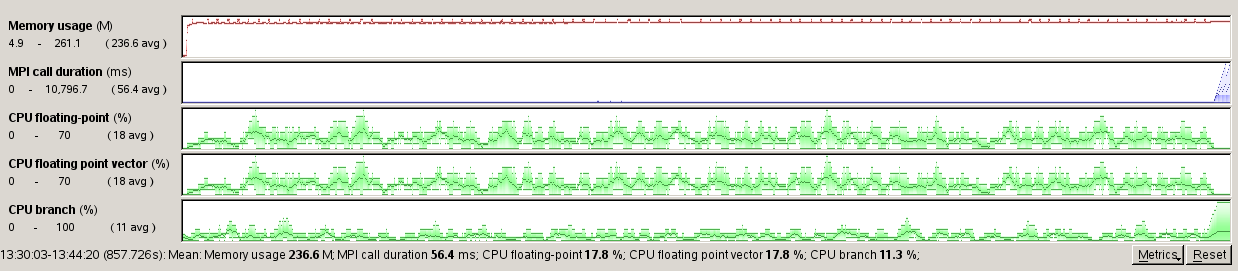
\includegraphics[width=\textwidth]{vec}

\end{frame}
\begin{frame}[fragile]{Logical CPU balance}
\vspace{20mm}
\begin{figure}
\begin{tikzpicture}[font=\footnotesize,xshift=-25mm,yshift=-17mm]
\begin{axis}[
scale only axis,
xmin=  1,xmax=240,
minor tick num =4,
every tick/.style={thick},
xlabel=hw threads, ylabel=time/s,
width=0.55\textwidth,
]
\addplot +[blue,thick] table[x index=0, y index=  1] {figures/vtune.dat};
\end{axis}
\end{tikzpicture}
\end{figure}
\vspace{20mm}
\par{15 MPI processes each 4 threads running on Xeon Phi}
\end{frame}

